\chapter{Evaluación de la red}
%\todo{evaluación de las red? Vamos a testear las funciones uqe has creado... DONE: Mejor que pruebas, si.}

Una vez que tenemos nuestra red funcionando y le hemos dado unos segundos para configurarse automáticamente vamos a realizar algunas pruebas sobre la misma para comprobar que la funcionalidad que hemos implementado funciona correctamente.

\section{Autoconfiguración de equipos.}

Vamos a probar que los nodos se autoconfiguran de forma automática como habíamos planeado. Para comprobar esto, al arrancar la red ejecutamos el comando \lstinline{ifconfig} en uno de los hosts de la red. Al principio aparece que no tiene asociada una dirección IP. Al cabo de unos segundos cuando la red ha convergido y ha dado tiempo a intercambiar todos los paquetes necesarios los hosts tienen dirección IP.

\begin{figure}[!h]
    \centering
    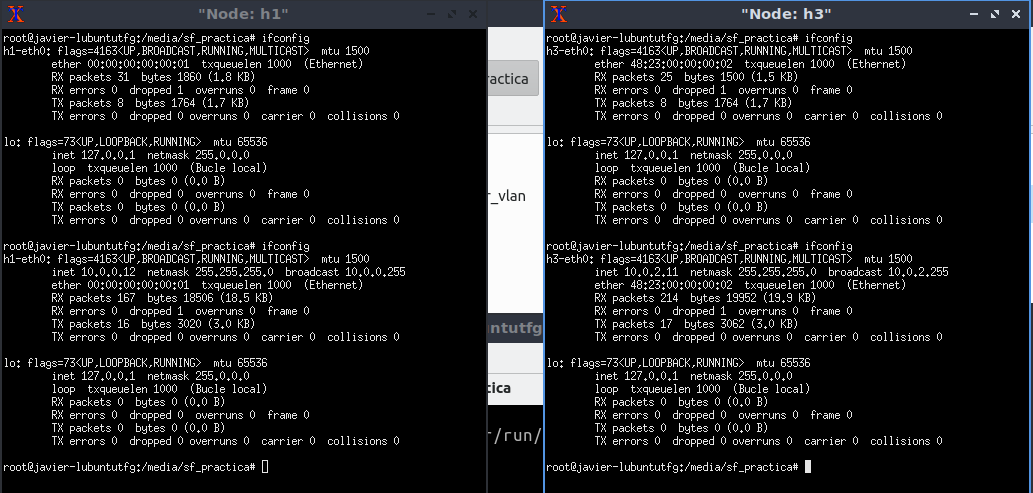
\includegraphics[width=\textwidth]{imagenes/figuras/autoconfig.png}
    \caption{Consolas de los nodos h1 y h3, pertenecientes a VLAN distintas mostrando su configuración al inicio y tras obtener una dirección IP}
    \label{fig:autoconfig}
\end{figure}

Como podemos observar en la figura \ref{fig:autoconfig} los nodos de la red obtienen del servidor DHCP una dirección IP en base a la VLAN a la que pertenecen. 

\section{Caída de enlaces}

Para comprobar la resiliencia de la red ante caídas de enlace y el correcto funcionamiento del protocolo STP vamos a probar a desactivar un enlace y hacer ping entre un nodo y el router.

\begin{figure}[!h]
    \centering
    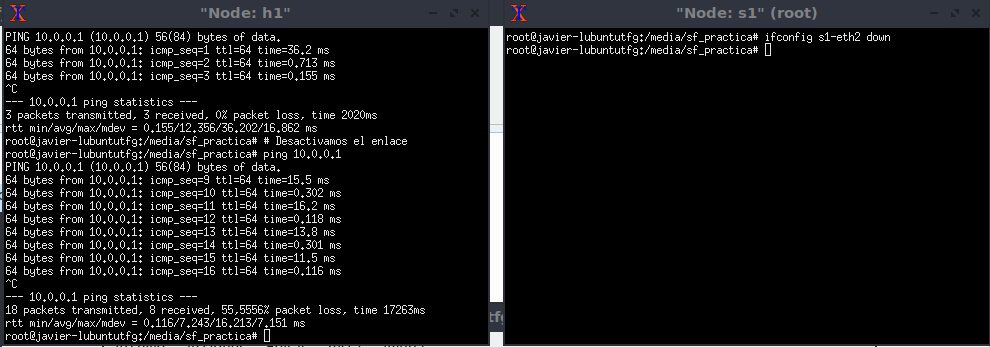
\includegraphics[width=\textwidth]{imagenes/figuras/caida_enlace.png}
    \caption{Ping entre dos dispositivos en un escenario de enlace caído}
    \label{fig:caida-enlace}
\end{figure}

Según se observa en la captura \ref{fig:caida-enlace} desconectamos una interfaz de red que conecta el switch 1 con el switch 3. El nodo es capaz de seguir accediendo al servidor a pesar del enlace caído ya que la red vuelve a ejecutar el algoritmo STP para eliminar bucles y conseguir conectividad completa de la red siempre que sea posible. En una red redundante como la que hemos diseñado tienen que caer todos los enlaces de un switch para que este se quede aislado del resto de la red.


\section{Evaluación de prestaciones}

Vamos a medir 3 parámetros básicos: la latencia media entre dispositivos, el retardo del primer paquete entre dos nodos y la velocidad pico alcanzable. Estas medidas serán ideales ya que nos encontramos en una red virtualizada. En un entorno real estas medidas pueden variar.

\subsection{Latencia media entre dispositivos}

Para conocer la latencia media de una manera aproximada vamos a ejecutar nmap desde el router dándole la orden de ejecutar pings a todos los dispositivos de la red. La línea a ejecutar es la siguiente:
\lstinline{nmap -sn 10.0.0,2.10-15} y su salida es esta:

\begin{lstlisting}[language=bash, label=lst:nmap-out, caption={Salida de nmap}]
root@javier-lubuntutfg:/media/sf_practica# nmap -sn 10.0.0,2.10-15
Nmap scan report for 10.0.0.10
Host is up (0.011s latency).
Nmap scan report for 10.0.0.11
Host is up (0.044s latency).
Nmap scan report for 10.0.0.12
Host is up (0.073s latency).
Nmap scan report for 10.0.2.10
Host is up (0.038s latency).
Nmap scan report for 10.0.2.11
Host is up (0.038s latency).
Nmap done: 12 IP addresses (5 hosts up) scanned in 26.83 seconds
\end{lstlisting}

Del listado \ref{lst:nmap-out} podemos aproximar una latencia media de 40,8 ms. Como nos parece mucho ping para una red local probamos a hacer pings individuales y hacer la media de las medias de ping. Lo hemos ejecutado con estos parámetros \lstinline{ping -q -c10 10.0.X.X}

\begin{lstlisting}[language=bash, label=lst:ping-out, caption={Salida de ping}]
root@javier-lubuntutfg:/media/sf_practica# ping 10.0.2.10 -q -c 10
--- 10.0.2.10 ping statistics ---
10 packets transmitted, 10 received, 0% packet loss, time 9198ms
rtt min/avg/max/mdev = 0.138/0.228/0.414/0.093 ms
--- 10.0.2.11 ping statistics ---
10 packets transmitted, 10 received, 0% packet loss, time 9174ms
rtt min/avg/max/mdev = 0.117/0.356/1.871/0.506 ms
--- 10.0.0.10 ping statistics ---
10 packets transmitted, 10 received, 0% packet loss, time 9183ms
rtt min/avg/max/mdev = 0.077/0.243/0.909/0.228 ms
--- 10.0.0.11 ping statistics ---
10 packets transmitted, 10 received, 0% packet loss, time 9184ms
rtt min/avg/max/mdev = 0.056/0.514/3.583/1.025 ms
--- 10.0.0.12 ping statistics ---
10 packets transmitted, 10 received, 0% packet loss, time 9030ms
rtt min/avg/max/mdev = 2.368/3.567/6.754/1.263 ms
\end{lstlisting}

Del listado anterior calculamos una \textbf{latencia media de 0,978 ms}. Véase además como es el último nodo el que ralentiza más la red. Comprobando la tabla de macs sabemos que ese es el nodo que simula estar conectado mediante un enlace inalámbrico. Además mininet-wifi simula una red wifi de tipo 802.11g, de tecnología bastante más antigua que el estándar actual 802.11.ac

\subsection{Tiempo para el primer paquete}

Observando los resultados anteriores vemos que hay paquetes de ping con una latencia muy superior a la media. observando una salida completa de ping entre dos nodos que no se han comunicado entre sí anteriormente (figura \ref{fig:ping-first}) podemos comprobar que el primer paquete tarda más tiempo en llegar. Esto se debe a que el primer paquete es procesado por el controlador de la red, mientras que los paquetes sucesivos ya tienen una regla coincidente en los switches y no tienen que pasar por el controlador.

\begin{figure}[!h]
    \centering
    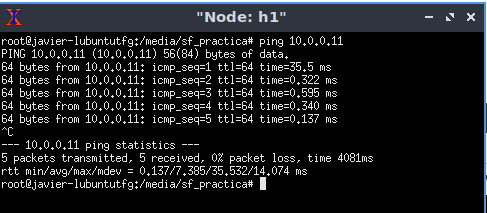
\includegraphics[width=\textwidth]{imagenes/figuras/ping_first.png}
    \caption{Ping entre dos dispositivos que no han tenido comunicación directa previamente.}
    \label{fig:ping-first}
\end{figure}

\subsection{Ancho de banda entre dos dispositivos}

Si ejecutamos iperf entre dos dispositivos podemos ver la velocidad del enlace entre ellos. En este caso vamos a medir la velocidad de enlace entre h3 y el router.

\begin{figure}[!h]
    \centering
    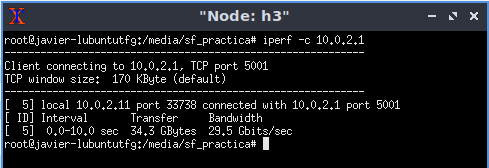
\includegraphics[width=\textwidth]{imagenes/figuras/iperf.png}
    \caption{Iperf ejecutándose entre dos nodos de la red.}
    \label{fig:iperf}
\end{figure}

La herramienta ha dado una velocidad entre ambos equipos de \textbf{29,5 Gb/s}. Esto se debe a que estamos en una red virtualizada. De hecho si probamos a hacer esta misma prueba con alguno de los nodos conectados mediante wifi veremos que alcanzamos una velocidad máxima del enlace inalámbrico (figura \ref{fig:iperf-wifi}) mucho menor: \textbf{9,65Mb/s}

\begin{figure}[!h]
    \centering
    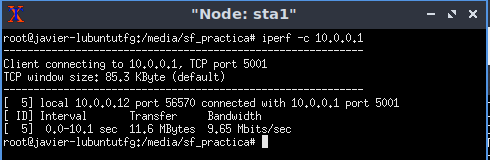
\includegraphics[width=\textwidth]{imagenes/figuras/iperf-wifi.png}
    \caption{Iperf ejecutándose entre dos nodos de la red, uno de ellos conectado de forma inalámbrica.}
    \label{fig:iperf-wifi}
\end{figure}

Medir parámetros básicos: latencia, tiempo al primer paquete, throughput medio.
